\documentclass[linenumbers, twocolumn]{aastex631}

\usepackage{graphicx}
\usepackage{amsmath}
\usepackage{amssymb}
\usepackage{newtxtext,newtxmath}
\usepackage{hyperref}
\usepackage{gensymb}
\usepackage{enumitem}

\newcommand{\vdag}{(v)^\dagger}
\newcommand\aastex{AAS\TeX}
\newcommand\latex{La\TeX}

\newcommand{\Msun}{\ensuremath{M_{\odot}}}
\newcommand{\Gyr}{\ensuremath{\textrm{Gyr}}}
\newcommand{\Myr}{\ensuremath{\textrm{Myr}}}
\newcommand{\yr}{\ensuremath{\textrm{yr}}}
\newcommand{\kpc}{\ensuremath{\textrm{kpc}}}
\newcommand{\pc}{\ensuremath{\textrm{pc}}}
\newcommand{\kms}{\ensuremath{\textrm{km}/\textrm{s}}}
\newcommand{\tocite}{\textcolor{blue}{cite}}
\newcommand{\FeH}{\ensuremath{[\textrm{Fe}/\textrm{H}]}}
\newcommand{\MgFe}{\ensuremath{[\textrm{Mg}/\textrm{Fe}]}}
\newcommand{\alphaFe}{\ensuremath{[\alpha/\textrm{Fe}]}}
\newcommand{\tform}{\ensuremath{t_{\textrm{form}}}}
\newcommand{\dex}{\ensuremath{\textrm{dex}}}
\newcommand{\Msunyr}{\ensuremath{\Msun/\textrm{yr}}}

\newcommand{\red}[1]{\textcolor{red}{#1}}

% \received{March 1, 2021}
% \revised{April 1, 2021}
%\accepted{\today}

\shorttitle{The Milky Way's Phoenix Phase}
\shortauthors{Beane}

\graphicspath{{./}{fig/}}

\begin{document}

\title{Rising from the Ashes: How the Milky Way Got Its Scars}

\author{Angus Beane}
\affiliation{Center for Astrophysics $|$ Harvard \& Smithsonian, Cambridge, MA, USA}

% \author{Lars Hernquist}
% \affiliation{Center for Astrophysics $|$ Harvard \& Smithsonian, Cambridge, MA, USA}

% \author{et al}

\begin{abstract}
    The elemental abundance distribution of stars encodes the history of the gas-phase abundance in the Milky Way. Without a large, unbiased sample of highly precise stellar ages, the exact timing and nature of this history must be \textit{inferred} from the abundances. In the two-dimensional plane of \alphaFe-\FeH, it is now clear that two separate populations exist -- the low-$\alpha$ and high-$\alpha$ sequences. Structure in the elemental abundance distribution can arise from many processes -- proposals include specific gas infall scenarios, radial migration, high-redshift clump formation, and various effects associated with galaxy mergers, among others. In this work, we demonstrate another possible avenue for structure formation with clear observational predictions. In this scenario, the Galaxy underwent a starburst followed by a brief (hundreds of Myr) quiescent phase -- i.e., the Galaxy underwent a post-starburst rejuvenation sequence at $z\sim2$. A natural consequence of the quiescent phase is that stars in the valley of the bimodality do not form because: (1) the absence of enrichment from high-mass stars leads to a rapid reduction in \alphaFe{}, and (2) any time the gas spends in the abundance valley is deemphasized in the present day distribution because the star formation rate is lower. With a set of idealized merger simulations, we demonstrate the feasibility of this proposal. This ``phoenix hypothesis'' predicts a $\sim300\,\Myr$ gap in stellar ages at a fixed \FeH{} and that stars which form directly after this gap would have lower \alphaFe{} than stars which form slightly ($\sim1\,\Gyr$) later.
  \end{abstract}
  
\keywords{Classical Novae (251) --- Ultraviolet astronomy(1736) --- History of astronomy(1868) --- Interdisciplinary astronomy(804)}


\section{Introduction} \label{sec:intro}
% What leads to distribution of heavy elements in a galaxy
Elements heavier than hydrogen are produced through nuclear fusion. After Big Bang Nucleosynthesis, this only occurs in compact objects such as supernovae, dying low mass stars, and neutron star-neutron star mergers \citep[e.g.][]{2023A&ARv..31....1A}. By necessity, stars inherit the constituitive properties of the gas from which they formed. Moreover, the surface abundance of most elements for most stars do not change over most of their lifetime. We therefore have the unique opportunity to examine the historical record of the gas-phase abundance of a galaxy by way of the distribution of the surface abundances of stars.

The enrichment of the gas-phase of a galaxy is determined by a complicated combination of physical processes - stellar evolution and supernovae, gas accretion, mergers, gas outflows from stellar and AGN feedback, metal mixing and diffusion, etc. Because the processes which give rise to this distribution are complex, there is almost certainly some structure in the stellar abundance distribution for every galaxy. However, it has only been definitively measured in the Milky Way (there is a claim of no measured structure in M31 by \citet{2024IAUS..377..115N}).

% How present-day stellar surface abundances are linked to history of gas-phase abundances

% Why alpha-elements are important
The distribution of elemental abundances is a high dimensional space \citep[e.g., 32 elements in][]{2024ApJ...961L..41J}. However, this space is highly degenerate, and so the effective number of dimensions is much smaller -- even possibly compressed to just \FeH{} and age \citep{2019ApJ...883..177N}. Two elements in particular have received particular interest - Fe and $\alpha$-elements. Type Ia and Type II supernovae are the main contributors of Fe and $\alpha$ enrichment. Fe is broadly produced in both types, and so its abundance is a proxy for the total metallicity of a star. On the other hand, $\alpha$-elements are mainly produced in Type II supernovae. The ratio of $\alpha$-elements to Fe (\alphaFe{}) is then a measure of the relative contributions of Type Ia and II SNe to the enrichment of a parcel of gas. It has therefore become common to compress the high-dimensional abundance space to the two dimensional \alphaFe{}-\FeH{} plane.

% Observed chemical bimodality in the Milky Way
It is now well-established that, in the Milky Way, a bimodality exists in the \alphaFe{}-\FeH{} plane \citep{1996ASPC...92..307G,1998A&A...338..161F,2004AN....325....3F,2006MNRAS.367.1329R,2011A&A...535L..11A,2012A&A...545A..32A,2014A&A...562A..71B,2014ApJ...796...38N,2020MNRAS.493.2952H}. This bimodality is typically separated into the high-$\alpha$ and low-$\alpha$ sequences. The high-$\alpha$ sequence is more centrally compact and vertically extended than the low-$\alpha$ sequence. 

% Different explanations of bimodality
Naturally, many different processes that could lead to structure in the abundance plane have been discussed in the literature. They can be separated into two broad classes: (1) structure arising from internal processes, and (2) structure arising from external processes. We will summarize these classes of explanations in turn.

An early explanation of the bimodality is the two-phase gas infall model \citep{1997ApJ...477..765C,2009IAUS..254..191C,2017MNRAS.472.3637G,2019A&A...623A..60S}. In this model, the thick disk first forms rapidly from an initial infall of gas. Because the typical SFR is high, these stars are $\alpha$-enhanced. In some variants, star formation halts completely before a second supply of pristine gas falls into the Galaxy. This dilutes the gas supply from which the thin disk forms more gradually. The thin disk is then more $\alpha$-poor because its associated SFR is lower.

A later argument by \citet{2021MNRAS.501.5176K} bears a passing resemblance to the two-infall model. Here, they argue that the two sequences follow from two phases of gas infall, except driven by stellar feedback instead of cosmological inflow. An initial bursty phase follows from the direct collapse of the gaseous halo. The disk has a high SFR leads to the formation of the high-$\alpha$ sequence. Feedback then halts the inflow, and a slower accretion of high-angular momentum and metal-rich gas commences, forming the low-$\alpha$ sequence.

Another mechanism to generate structure in the abundance plane was pointed out by \citet{2009MNRAS.396..203S}, further developed by \citet{2021MNRAS.507.5882S,2023MNRAS.523.3791C}, and explored by \citet{2011ApJ...737....8L,2021MNRAS.508.4484J}. This model claims that, since stars are thought to migrate from their birth radius, there will be stars throughout the entire disk that formed in the inner disk. These $\alpha$-enhanced stars will then form the high-$\alpha$ sequence. This model and its variants also match some chemodynamic properties of the disk. One salient feature of these models is that the bimodality can result from a smooth star formation history.

Yet another explanation invoking an internal process is that the formation of clumps at high redshift are responsible for both the chemistry and dynamics of the high-$\alpha$ sequence \citep{2019MNRAS.484.3476C,2020MNRAS.492.4716B,2021MNRAS.502..260B,2023ApJ...953..128G}. Instabilities are thought to form clumps in gas-rich disks, and such clumps are seen at intermediate redshifts \citep[$z\sim2$;][]{2005ApJ...627..632E,2007ApJ...658..763E}. These clumps then self-enrich, forming $\alpha$-enhanced stars. The high-$\alpha$ sequence stops forming once the gas fraction is low enough for the instabilities to no longer arise. This model predicts that the high-$\alpha$ and low-$\alpha$ sequences form simultaneously.

Next, we turn to models which argue the bimodality results from some external influence. Early arguments were made that both the $\alpha$-enhancement of the disk and the thickening of the disk can result from gas-rich mergers \citep{2004ApJ...612..894B,2005ApJ...630..298B,2007ApJ...658...60B,2010MNRAS.402.1489R}.\footnote{See also \citet{2009MNRAS.400.1347C} for an argument invoking semi-analytic models.} These mergers lead to an enhanced SFR which leads to the $\alpha$-enhancement of the thick disk.

In cosmological simulations, which naturally include early gas-rich mergers, the situation is not as clear. Early work by \citet{2012MNRAS.426..690B} found a general separation between the thin and thick disk, though other authors found a smooth evolution \citep{2013A&A...558A...9M}. \citet{2018MNRAS.474.3629G} found what they referred to as a chemical dichotomy, and argued that it can come from either gas-rich mergers as described before or a ``compaction'' of the disk (we will return to this point in Section~\ref{ssec:cosmo}). Other authors highlight the metal content of the infalling gas, stating that the metal-poor gas associated with satellites can suddenly dilute or reset the disk's metallicity \citep{2020MNRAS.491.5435B,2024MNRAS.528L.122C}

The merger explanation of the bimodality is highly synergistic with our picture of the hierarchical assembly of the stellar halo \citep{2005ApJ...635..931B}. Indeed, there is strong evidence that the Milky Way underwent a significant merger with the so-called Gaia-Sausage-Enceladus satellite \citep[GSE;][]{2018MNRAS.478..611B,2018Natur.563...85H,2020ApJ...901...48N}. This merger is thought to have occurred $\sim8-10\,\Gyr$ ago \citep[see also][]{2020ApJ...897L..18B}.

Claims in the literature on the stellar mass of GSE vary widely. Early estimates argued from $6\times10^8$ up to even $10^{10}\,\Msun$ \citep{2018MNRAS.478..611B,2018Natur.563...85H,2019MNRAS.484.4471F,2019MNRAS.487L..47V,2019MNRAS.488.1235M,2020MNRAS.493.5195D,2020MNRAS.497..109F}. Later estimates have been more conservatives with estimates from a mass of $3\times10^8\,\Msun$ to $10^9\,\Msun$ \citep{2019MNRAS.482.3426M,2020MNRAS.492.3631M,2021ApJ...923...92N,2022AJ....164..249H}, and even as low as $1.5\times10^8\,\Msun$ \citep{2023MNRAS.526.1209L}.

In this work, we explored an idealized merger simulation which resembles the merger between the Milky Way and GSE. We found that in certain configurations, which have only minor differences in their orbit, a bimodal distribution of stellar abundances in the \alphaFe{}-\FeH{} plane is produced. This is shown in Figure~\ref{fig:fig1}. The configurations which produce a bimodality are associated with a starburst followed by a quiescent phase followed by rejuvenation $\sim300\,\Myr$ later.

In Section~\ref{sec:methods}, we describe our setup. In Section~\ref{sec:results}, we present the main results of our simulations. In Section~\ref{sec:discussion}, we discuss and interpret our results, as well as connections to previous and future work, before concluding in Section~\ref{sec:conclusion}. Throughout this work we refer to the standard native time unit $\kpc/\left(\kms\right)$ as \Gyr{} for convenience.

\begin{figure*}
  \centering
  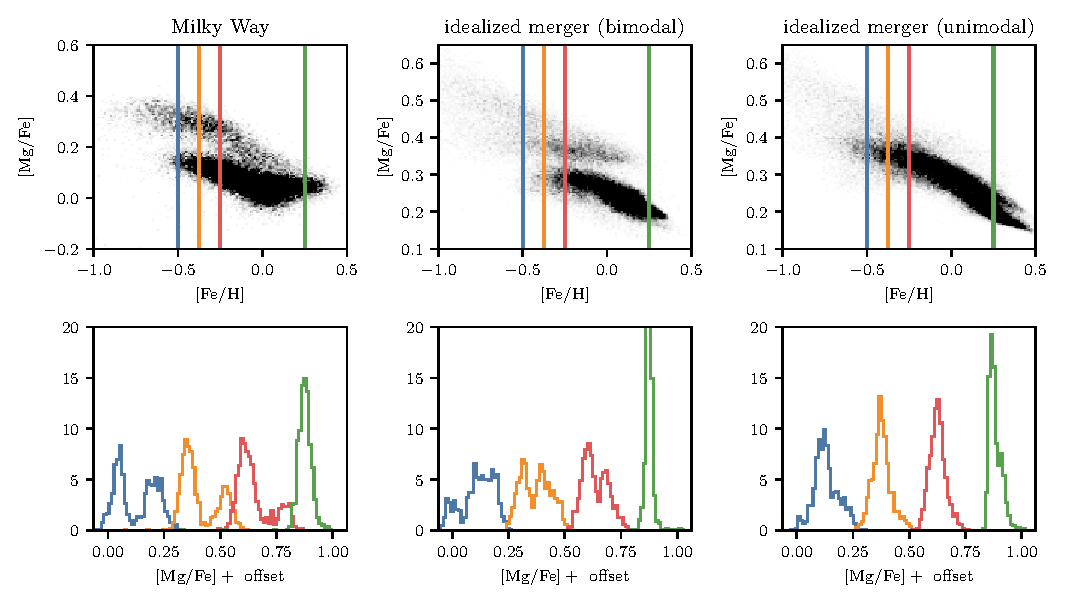
\includegraphics[width=\textwidth]{figure1.pdf}
  \caption{\textbf{The abundance bimodality seen in the Milky Way can be reproduced in some idealized merger simulations.} In the upper panels, we show the distribution of stars in the \MgFe-\FeH plane. The left panel shows the observed distribution in the Milky Way from ASPCAP DR17 \citep[][J.A.~Holtzman et al., in preparation]{2016AJ....151..144G}, while the right two panels show two idealized merger simulations. The idealized merger simulations are nearly identical, except that the bimodal simulation has a starting radius of $129\,\kpc$, while the unimodal simulation has a starting radius of $142\,\kpc$. We emphasize that the labels ``unimodal'' and ``bimodal'' are of the \textit{outcome} of the simulation, and do not reflect a particular choice in the setup. The bottom panels show the distribution of \MgFe at fixed \FeH. The colors indicate the fixed \FeH values, which are $-0.5$, $-0.25$, $0$, and $0.25$. The Milky Way (left panels) exhibits a strong bimodal distribution of \MgFe at various \FeH. The idealized merger simulation marked as bimodal (center panels) also exhibits a bimodal distribution of \MgFe, though the structure is not as strongly defined. The idealized merger simulation marked as unimodal exhibits only weak structure, if any at all.}
  \label{fig:fig1}
\end{figure*}

\section{Methods}\label{sec:methods}
\subsection{Isolated Setup}\label{ssec:iso_setup}
In isolation, each of the central and satellite galaxies are a compound halo setup, with a Hernquist dark matter halo and a gaseous halo with a $\beta$-profile:
\begin{equation*}
\rho = \rho_0 \left[1 + \left(\frac{r}{r_c}\right)^2\right]^{-\frac{3\beta}{2}}
\end{equation*}
The total mass within the virial radius is kept fixed, and the mass of the dark matter halo and central density of the gaseous halo are chosen to satisfy a given baryon fraction $f_b$. The dark matter halo is initialized to be in gravitational equilibrium with the total potential. The gaseous halo is in gravito-hydrostatic equilibrium, where the temperature is allowed to vary as a function of radius. The azimuthal velocity of the gaseous halo is given as a fraction of the circular velocity. There is no initial stellar disk or bulge, and the gas is initially metal-free. Thus, all star particles and metals are formed self-consistently.

We manually varied the different model parameters until we arrived at a setup that resulted in reaosnable galaxies (as determined by their stellar mass). For the central (Milky Way) galaxy, we set $M_{200}=5\times10^{11}\,\Msun$, $c_{200}=4.1$, $\beta=0.8$, $r_c=9\,\kpc$, $f_b=0.08$, and $v_{\phi}/v_{\textrm{c}}=0.2$, where $c_{200}$ is the concentration and $v_{\phi}/v_{\textrm{c}}$ is the azimuthal velocity of the gaseous halo (as a fraction of the circular velocity). For the satellite (GSE) galaxy, we set $M_{200}=2.2\times10^{11}\,\Msun$, $c_{200}=4.33$, $\beta=0.8$, $r_c=6.5\,\kpc$, $f_b=0.06$, and $v_{\phi}/v_{\textrm{c}}=0.4$.

The stellar mass build-up of our Milky Way-like and GSE-like galaxies is given in Figure~\ref{fig:mass_size}. The upper panel shows the stellar mass history. We attempt to match the expected mass of the present-day thick disk \citep[$\sim6\times10^9\,\Msun$, horizontal blue dashed line][]{2016ARA&A..54..529B} at an evolution time of $\sim3\,\Gyr$ (corresponding to $z\sim2$, vertical dashed gray line).\footnote{Of course, this neglects the significant mass contribution of the bulge, which presumably formed earlier. However, our setup does not form a strong spheroidal component. Using the trick in e.g. \citet{2022MNRAS.515.1524Z}, we take the bulge mass to be twice the counterrotating stellar mass. At $3\,\Gyr$ in the isolated Milky Way-like galaxy, the bulge mass is $\sim7\times10^{8}\,\Msun$, or $\sim13\%$ of the total mass. The Milky Way's bulge is  $\sim1.5\times10^{10}\,\Msun$, although there is strong debate about just how much of the bulge is a classical bulge which formed before the disk \citep{2016ARA&A..54..529B}. In any case, we did not attempt to match any particular property of the bulge, though one could promote bulge formation by reducing the rotation of the gas in the inner region.} We get reasonably close at $\sim5\times10^9\,\Msun$ (blue line). For GSE, we use the best-fit mass from the $N$-body simulations of \citet{2021ApJ...923...92N} -- $5\times10^8\,\Msun$ (horizontal dashed orange line). For this, we slightly overestimate (orange line).

As for the galaxy sizes, there is significant spread amongst the real galaxy population, and the sizes are thought to be influenced by the merger history not present in our setup \citep[e.g.][]{2014ApJ...788...28V}. We note that the sizes of each simulated galaxy (lower panel) are within the range of observed galaxy sizes. For the Milky Way, we know the thick disk has scale length of $\sim2\,\kpc$, which converts to a half-mass radius of $\sim3.36\,\kpc$. At $\sim3\,\Gyr$, our Milky Way-like galaxy has a half-mass radius of $\sim2\,\kpc$. Curiously, after $3\,\Gyr$, the size of the Milky Way-like galaxy continues to grow while the GSE galaxy's size remains constant for the duration of the simulation. 

\begin{figure}
    \centering
    \includegraphics[width=\columnwidth]{mass_size.pdf}
    \caption{The mass and size evolution of the central (Milky Way, blue) and satellite (GSE, orange) galaxies. The mass is taken to be the stellar mass within twice the half-mass radius, and the size is taken to be the half-mass radius. In the upper panel, we also show as a horizontal line the mass of the Milky Way's disk and GSE from the best-fit model of \citet{2021ApJ...923...92N}. This comparison is taken to be made at $3\,\Gyr$ (vertical dashed line), our proxy for $z\sim2$. A precise match is not attempted given the wide ranging uncertainties.}
    \label{fig:mass_size}
  \end{figure}

\subsection{Orbital Configuration}\label{ssec:orbit_setup}
In order to combine the galaxies, we follow \citet{2021ApJ...923...92N}, and place the satellite galaxy on a retrograde orbit. In the fiducial simulation of \citet{2021ApJ...923...92N}, the satellite is placed at the virial radius ($129\,\kpc$), with the virial velocity ($129\,\kms$), and with a circularity of $0.5$. To test minor changes to the orbit, we ran a grid of simulations with $\pm10\%$ in each the starting radius and velocity, and $\pm0.1$ in the circularity, for a total of $27$ simulations. We performed each simulation for a duration of $8\,\Gyr$.

Some of the simulations in this orbital grid resulted in bimodal abundance distributions, while some had little to no structure in the abundance distribution plane. We show the abundance plane for all $27$ simulations in Appendix~\ref{app:allsims}, but for the main body of this work we consider two representative simulations in detail. For the bimodal simulation, we chose the simulation with $R_0=142\,\kpc$, $V_0=116\,\kms$, and $\eta=0.4$. For the unimodal simulation, the parameters are the same except that $R_0=129\,\kpc$.

\subsection{Feedback and Enrichment Model}\label{ssec:gfm}
Our feedback model is most closely related to that used in the Illustris TNG simulation suite \citep{2013MNRAS.436.3031V,2017MNRAS.465.3291W,2018MNRAS.473.4077P}. In this model, gravity and magnetohydrodynamics are solved using a \citet{1986Natur.324..446B} tree coupled to a second order finite volume fluid solver in AREPO \citep{2010MNRAS.401..791S,2016MNRAS.455.1134P}. Stellar feedback is included through a subgrid wind particle model \citep{2003MNRAS.339..289S}. AGN feedback follows a dual kinetic and thermal mode for low- and high-accretion rates \citep{2017MNRAS.465.3291W}.

In this work, we made some simplifications to this model in order to aid interpretation. First, we ignore magnetic fields. This was motivated by an initial desire to understand the CGM accretion rates in terms of idealized cooling flow solutions, but we did not revisit turning them back on. In any case, it is not clear if the magnetic fields would be realistically generated given our initial setup. Second, we use a gentler wind feedback model as described in \citet{2019MNRAS.489.4233M}. Because our setup includes both an initially steep central potential and no steady-state disk, a stronger feedback model would require a higher central gas density to achieve a reasonable SFH which introduced its own set of instabilities.

In this model, star particles synthesize elements through three different channels for which we cite the relevant yield tables: SNe Ia \citep{1997NuPhA.621..467N}, SNe II \citep{1998A&A...334..505P,2006ApJ...653.1145K}, and AGB stars \citep{2010MNRAS.403.1413K,2014MNRAS.437..195D,2014ApJ...797...44F}. Recall that star particles are simple stellar populations (i.e., a collection of stars with the same age and chemical composition). Each star particle continuously injects metals into its surroundings in the following sequence\footnote{The kinetic/thermal feedback component is handled through the wind generation, which is completely separate in this model.}:
\begin{enumerate}
    \item $t\lesssim10\,\Myr$: no metal injection as the first supernova ($M\sim100\,\Msun$) has not gone off
    \item $10\,\Myr \lesssim t \lesssim 40\,\Myr$: metal injection as $8\,\Msun<M<100\,\Msun$ stars die as Type II SNe
    \item $t\gtrsim40\,\Myr$: metal injection from Type Ia SNe and AGB stars
\end{enumerate}
There are a few things to note: (1) The exact timings are metallicity-dependent. (2) The \MgFe{} of ejected gas from Type II SNe are mass/time-dependent, with more massive stars contributing more Mg than less massive stars. (3) Type II SNe contribute the vast majority of Mg ($\sim10\times$ AGB and $\sim100\times$ Type Ia SNe). Type Ia and Type II SNe contribute approximately equal amounts of Fe ($\sim3\times$ AGB). See Figure~1 from \citet{2018MNRAS.473.4077P}. (4) The number of Type Ia SNe is greater for a younger stellar population, with a power law relationship $\propto t^{-1.12}$.

\subsection{Observed Abundances}\label{ssec:obs_abund}
Our aim in this work is to demonstrate the feasibility of a mechanism for structure formation in the abundance plane. We are only making a qualitative comparison to data. Therefore, we use the ASPCAP DR17 catalog of stellar abundances (\citet{2016AJ....151..144G}; J.A.~Holtzman et al., in preparation), which is publicly available, well-established, and widely used.

We first make some quality cuts, as well as restricting our sample to dwarfs \red{check}. We require:
\begin{itemize}[noitemsep]
    \item $\textrm{SNR} > 200$,
    \item $\textrm{VSCATTER} < 1\,\kms$,
    \item STARFLAG not set,
    \item $\varpi/\sigma_{\varpi} > 1$,
    \item $\log{g} < 3.5$,
    \item $\sigma_{\log{g}} < 0.2$,
\end{itemize}
where $\varpi$ is the parallax. We use the parallax, proper motion, and radial velocity from Gaia EDR3 \citep{2016AA...595A...1G, 2021AA...649A...1G, 2021AA...649A...2L, 2021AA...653A.160S}.

We next make a selection on the angular momentum of stars in order to make a solar neighborhood selection. We assume the solar radius and azimuthal velocity are $R_0=8\,\kpc$ and $V_0=220\,\kms$ \red{cite}, and select stars which have $L_z$ within $10\%$ of the solar angular momentum. We further require that $\left|z\right| < 3\,\kpc$.

As is typically done, we use \FeH{} as an indicator of the total metallicity of a star. We use Mg alone as a representative of the $\alpha$-elements.

\subsection{Solar Neighborhood in Simulations}\label{ssec:solarneigh}
When comparing galaxy simulations to the observed solar neighborhood, some ambiguity arises in how to make a ``solar neighborhood-like'' selection of star particles. Naturally, this selection is dependent on the posed question. In this work, this is the formation of the abundance bimodality. The Sun is known to sit near the end of the thick disk, where the thick and thin disk have comparable surface densities (the ratio of thick-to-thin is $\sim12\%$ \red{cite}). As a result, the abundance bimodality appears most strongly near the Sun -- further inwards the high-$\alpha$ sequence is more dominant and further outwards the high-$\alpha$ sequence vanishes \red{cite}.

We mimic our selection of the solar neighborhood by also making a cut in angular momentum. However, in the simulation, the high-$\alpha$ disk is more compact than in the Galaxy. Therefore, in order to strike a balance between the low-$\alpha$ and high-$\alpha$ disks, we used an angular momentum cut which is $20\%$ that of our assumed solar angular momentum. In particular, we select all star particles with angular momenta within $30\%$ of $0.2\times8\,\kpc\times220\,\kms$ -- as well as requiring $\left| z \right| < 3\,\kpc$.

This choice of angular momentum may seem unrealistic. However, it corresponds to roughly selecting star particles with radii between $2$ and $5\,\kpc$. As discussed in Section~\ref{ssec:iso_setup}, our Milky Way-like galaxy is more compact than the Milky Way's thick disk.


\section{Results}\label{sec:results}
\subsection{Surface Density Projections}\label{ssec:projections}
Before dissecting the simulated galaxies in detail, we first take a look at the surface density projections of the gas and stars in the central region, situated on the central galaxy in the bimodal simulation. This is shown in Figure~\ref{fig:projections}. In each grouping of four, the bottom and top rows show the face-on and edge-on views, respectively. The left and right columns show the gas (blue) and stellar (orange) surface density, respectively. Each panel is oriented with respect to the stellar angular momentum of the final snapshot ($t=8\,\Gyr$). The angular momentum is computed using all star particles within the half-mass radius.

We can see that the galaxy grows in size after the merger. Additionally, the galaxy's orientation continues to change even within the last $3\,\Gyr$. The final galaxy is oriented $\sim126\degree$ with respect to the initial orientation of the central galaxy's gas halo. The dynamical and kinematic consequences of such a gas-rich merger is beyond the scope of our current work.

\begin{figure*}
  \centering

    \gridline{\fig{all_L30/all_L30_frame60.pdf}{0.3\textwidth}{}
              \fig{all_L30/all_L30_frame70.pdf}{0.3\textwidth}{}
              \fig{all_L30/all_L30_frame80.pdf}{0.3\textwidth}{}
              }
    \gridline{\fig{all_L30/all_L30_frame90.pdf}{0.3\textwidth}{}
              \fig{all_L30/all_L30_frame100.pdf}{0.3\textwidth}{}
              \fig{all_L30/all_L30_frame110.pdf}{0.3\textwidth}{}
              }
    \gridline{\fig{all_L30/all_L30_frame120.pdf}{0.3\textwidth}{}
              \fig{all_L30/all_L30_frame200.pdf}{0.3\textwidth}{}
              \fig{all_L30/all_L30_frame320.pdf}{0.3\textwidth}{}
              }
  % \includegraphics[width=\textwidth]{surfdens.pdf}
  \caption{Frames from a movie showing a surface density projection of the bimodal simulation over time. In each frame, the left/right (blue/orange) column shows the gas/star surface density. The upper/lower panels show the edge-on and face-on view. Every panel is oriented with respect to the final ($t=8\,\Gyr$) snapshot. The side-length of each panel is $30\,\kpc$, and the image is a projection through a box with the same side-length. The colormap for the gas ranges from $1$ to $10^2\,\Msun/\pc^2$, while for the stars ranges from $1$ to $10^4\,\Msun/\pc^2$. (A full movie, also for the unimodal and isolated simulations, is here \red{TBD}.)}
  \label{fig:projections}
\end{figure*}

\subsection{Abundance Distribution}\label{ssec:abundplane}
In Figure~\ref{fig:fig1}, briefly discussed in Section~\ref{sec:intro}, we show the abundance distribution of the Milky Way as well as two of our idealized merger simulations in the upper panels. A number of our idealized simulations exhibit either a bimodal or unimodal abundance distribution, and so we have selected two representative examples. The simulation labeled bimodal had orbital parameters of $R_0=142\,\kpc$, $V_0=116\,\kms$, and $\eta=0.4$. The unimodal simulation is identical, except that $R_0=129\,\kpc$. The bimodal and unimodal labels are of the outcome of the simulation, and do not reflect any particular choice made in their setup.

There are, of course, differences between the bimodal simulation and the Milky Way. First, the scaling in \MgFe{} is different -- in the simulation, the low-$\alpha$ sequence lies at $\sim0.2$, while in the Milky Way it is at about $\MgFe\sim0$. Second, in the Milky Way the high-$\alpha$ sequence neatly joins the low-$\alpha$ sequence at $\FeH\sim0$, while in the simulation the two actually diverge more at higher \FeH{}. Finally, at high \FeH{} the distribution bends upwards while in the simulation it bends downwards.

In the lower panels of Figure~\ref{fig:fig1}, we show the distributions of \MgFe{} at different fixed \FeH{}. The (blue, orange, red, green) lines show the \MgFe{} distribution at a \FeH{} of ($-0.5$, $-0.25$, $0$, $0.25$), in bins of width $0.05\,\dex$. The distributions of \MgFe{} are offset (but not rescaled) so that they do not overlap. Here, the bimodality seen in the Milky Way is quite striking at lower metallicities. The peaks are well-separated, by $\sim0.2\,\dex$. In the bimodal simulation, the distribution is still clearly bimodal, but the peaks are less well-separated, by $\sim0.1\,\dex$. In the unimodal simulation, there is a hint of some structure at $\FeH \gtrsim 0.25$, but there is not a strong multimodal structure.

\subsection{Build up of the Abundance Plane}\label{ssec:abundplane_build}
Next, we examine the build up of the abundance plane. First, in Figure~\ref{fig:before_after}, we show the abundance plane at various points along the merger. We have divided the history of the merger into ``before'' ($t < 1.5\,\Gyr$), ``during'' ($1.5\,\Gyr < t < 2.5\,\Gyr$), and ``after'' ($t > 2.5\,\Gyr$). These times have been chosen somewhat by the orbital history and somewhat by visually inspecting the simulation, and so these deliniations are, to an extent, arbitrary. Nonetheless, it is clear that the high-$\alpha$ sequence forms before and during the merger (middle panels), and that the low-$\alpha$ sequence forms after the merger (right panel). We show a dashed line given by $-0.1\times\FeH + 0.31$, which is a crude way of separating the high- and low-$\alpha$ sequence.

It is informative to examine the star formation history (SFH) split into the high- and low-$\alpha$ sequences at a fixed \FeH{}, shown in Figure~\ref{fig:before_after_sfh}. The high- and low-$\alpha$ sequences (blue and orange) are defined as the star particles lying above and below the dashed line in Figure~\ref{fig:before_after}, respectively. We show this only in a narrow bin of width $0.1\,\dex$ at $\FeH\sim0$. We chose this value of \FeH{} because here the valley of the bimodality is deepest (see Figure~\ref{fig:fig1}). One can see a very clear separation in time between the high- and low-$\alpha$ sequences, with the high-$\alpha$ sequence forming before the low-$\alpha$ sequence.\footnote{There is a small amount of low-$\alpha$ formation at the very end of the high-$\alpha$ sequence, but this can be understood as simply an inadequacy in our simple way of separating the two sequences. Alternatively, one could assert that the separation in time is the real delineation between the two sequences, and that the boundary in the abundance plane has only mild contamination.} Furthermore, there is a brief period of $\sim300\,\Myr$ between the two sequences where no stars have formed.

It can also be shown that the exact timing of this quiescent period is metallicity-dependent. We show the same SFH in Figure~\ref{fig:before_after_sfh_by_iron}, but at varying bins in \FeH{} of $-0.5$, $-0.25$, and $0$ (blue, orange, and red, respectively). For clarity, we do not separate the SFHs by the high- and low-$\alpha$ sequences, but have verified that the same demarcation arises as in Figure~\ref{fig:before_after_sfh}. Here, we can see that at $\FeH=-0.5$ the quiescent period begins $\sim250\,\Myr$ earlier than at $\FeH=0$.

\subsection{\alphaFe{} Behavior Associated with Quiescence}
We now examine more closely the natural suspicion that the quiescent phase in Figure~\ref{fig:before_after_sfh} is responsible for the bimodal structure in Figure~\ref{fig:before_after}. In Figure~\ref{fig:SFR_alpha}, we show the SFR (blue lines) of each of the bimodal and unimodal galaxies (left and right panels, respectively) as well as the median \MgFe{} of the gas (orange lines) in a bin centered on $\FeH{}=-0.1$ with width $0.05\,\dex$. The SFR is shown for the entire galaxy ($r<15\,\kpc$) while the median \MgFe{} is shown for $2\,\kpc<r<5\,\kpc$.\footnote{The solar neighborhood-like selection of stars (discussed in Section~\ref{ssec:solarneigh}) mostly selects stars at $2\,\kpc<r<5\,\kpc$. We choose to plot the median \MgFe{} of the gas at these radii, since it is roughly that gas which is forming stars that ends up in our sample. On the other hand, we choose to show the SFR for the entire galaxy, as the enrichment from that star formation affects the entire galaxy at this epoch.}

The merger appears to induce a starburst, where the SFR rises from $\sim3.5\,\Msunyr$ at $\sim1\Gyr$ to a peak of $\sim12\,\Msunyr$ at $\sim2\,\Gyr$. This starburst is then followed by a quiescent period, with a minimum SFR of $\sim1\,\Msunyr$ and a duration of $\sim500\,\Myr$. The dip in SFR is not as pronounced as it was when we plotted the SFH at a particular iron (Figure~\ref{fig:before_after_sfh}). This quiescent period is associated with a drop in \MgFe{} from $\sim0.35$ to $\sim0.2\,\dex$ in only $\sim250\,\Myr$. Once the SFR recovers $\sim500\,\Myr$ later, \MgFe{} again rises, but only to $\sim0.28\,\dex$.

This behavior is absent in the unimodal simulation (right panel) -- while there is a starburst, it does not display a period of suppressed star formation, and there is no associated drop in \MgFe{}. It does still have a period of enhanced star formation, but this is actually coincident with an enhancement in \MgFe{}. This sequence of events is further emphasized in Figure~\ref{fig:alpha_vs_tform}, which shows a transparent scatter plot of \MgFe{} as a function of formation time. In the bimodal simulation, there is a clear gap in \MgFe{} during the period of quiescence followed by the brief formation of $\alpha$-deficient stars. In the unimodal simulation, on the other hand, there is no gap and instead a brief formation of $\alpha$-enhanced stars.

\subsection{Cause of Quiescence}\label{ssec:cause_qui}
Why there is a quiescent period in the bimodal simulation but not the unimodal simulation probably has to do with some transient, stochastic property of the gas in and around the galaxy. In some states, the AGN is better able to quench the galaxy than in others. Verifying this further is beyond the scope of this work, but we show some evidence of the association in Appendix~\ref{app:cause_qui}.

This outcome suggests that a merger alone is not sufficient in order to generate a bimodality. Rather, the merger must induce a quenching phase. Whether this occurs depends both on the properties of the merger but also on the state of the central galaxy itself and whether it can launch AGN-driven winds that result in significant gas removal. Our work would argue for some stochasticity in whether a particular merger leads to such quenching.

\begin{figure*}
  \centering
  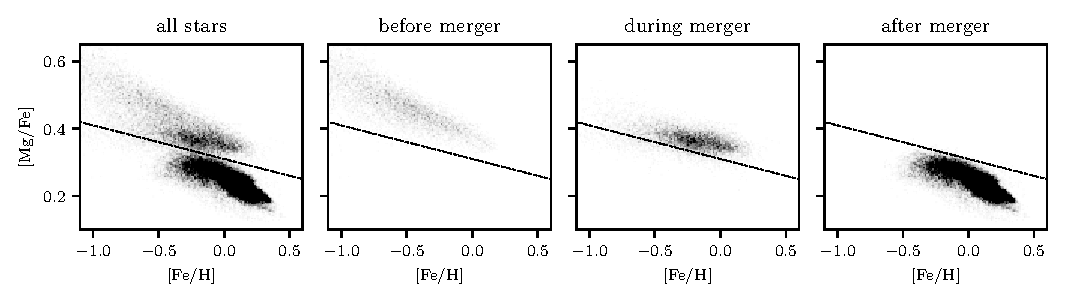
\includegraphics[width=\textwidth]{before_after.pdf}
  \caption{\textbf{The high-$\alpha$ sequence forms before the merger, the low-$\alpha$ sequence forms after the merger.} This plot shows the sequence of events leading to the build-up of the low- and high-$\alpha$ sequences for our fiducial bimodal simulation. We have separated the high- and low-$\alpha$ sequences by a dashed line at $-0.1\FeH + 0.31$, which was chosen by eye to lie in the trough. The left panel shows all star particles in our solar neighborhood cut. The middle left panel shows the star particles that form before the merger ($\tform < 1.5\,\Gyr$), which form a weak sequence of star particles at the lowest \FeH and highest \MgFe. The middle right panel shows the star particles that form during the starburst ($1.5\,\Gyr < \tform < 2.5\,\Gyr$). These star particles form the portion of the high-$\alpha$ sequence closest to the trough, and the density of star particless is higher than those that form before. The right panel shows the star particles which form after the merger ($\tform > 2.5\,\Gyr$). These star particles form almost entirely below the trough.}
  \label{fig:before_after}
\end{figure*}

\begin{figure}
  \centering
  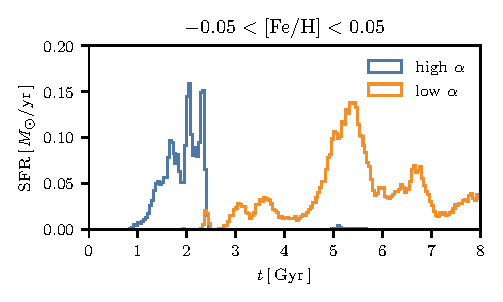
\includegraphics[width=\columnwidth]{before_after_sfh.pdf}
  \caption{\textbf{At fixed metallicity, the low- and high-$\alpha$ sequence are cleanly separated in time by an intervening quiescent period.} Here we show the star formation history of the high- and low-$\alpha$ sequences. The blue (low-$\alpha$) and orange (high-$\alpha$) histograms correspond to the dashed line cut made in the \MgFe{}-\FeH{} plane in Figure~\ref{fig:before_after}, at a fixed metallicity of $\FeH=0$ with width $0.05\,\dex$. One can see that there is a nearly perfect separation in time between the formation of the high-$\alpha$ and low-$\alpha$ sequences by a quiescent period lasting $\sim300\,\Myr$. There is a small amount of contamination at the end of the high-$\alpha$ sequence which can be attributed to the inadequacy of the linear cut model of the two sequences.}
  \label{fig:before_after_sfh}
\end{figure}

\begin{figure}
  \centering
  \includegraphics[width=\columnwidth]{before_after_sfh_by_iron.pdf}
  \caption{\textbf{The timing of the quiescent period which divides the high- and low-$\alpha$ sequences is metallicity dependent.} The star formation history of stars at various fixed metallicities ($\FeH=0$, $-0.25$, and $-0.5\,\textrm{dex}$) in bins of width $0.05\,\dex$. As in Figure~\ref{fig:before_after_sfh}, there is a quiescent period period which separates the formation of the low- and high-$\alpha$ sequence. However, the timing of the quiescent period is metallicity-dependent. It occurs earlier at lower metallicities, by $\sim250\,\Myr$ for the metallicities shown in this plot.}
  \label{fig:before_after_sfh_by_iron}
\end{figure}

\begin{figure*}
  \centering
  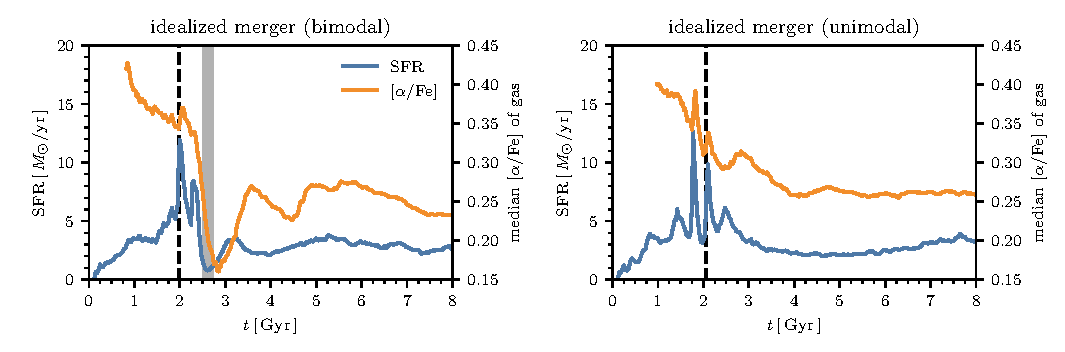
\includegraphics[width=\textwidth]{SFR_alpha.pdf}
  \caption{\textbf{A global suppression of star formation is associcated with a decrease in \MgFe{}, which is seen in the bimodal simulation but not in the unimodal simulation.} Here, we show both the SFR of the central galaxy ($r<15\,\kpc$) and the median \MgFe{} for gas at $2\,\kpc<r<5\,\kpc$ at a fixed \FeH{} bin centered on $0$ with width $0.05\,\dex$. The left panel shows the bimodal simulation while the right panel shows the unimodal simulation. A vertical dashed line at $2\,\Gyr$ in each plot indicates the approximate time of the merger, but before complete coalescence. In the left panel, a shaded region from $2.5\,\Gyr$ to $2.75\,\Gyr$ indicates the approximate period of quiescence shown in Figure~\ref{fig:before_after_sfh}. This suppression of star formation is associated with a sudden drop in the median \MgFe{} of the gas. Neither the suppression of star formation nor the drop in \MgFe{} are seen in the unimodal simulation.}
  \label{fig:SFR_alpha}
\end{figure*}

\begin{figure}
  \centering
  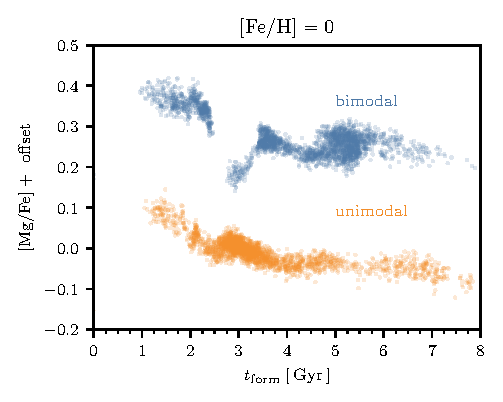
\includegraphics[width=\columnwidth]{alpha_vs_tform.pdf}
  \caption{\textbf{In the bimodal simulation, a gap in stellar ages is briefly followed by the formation of $\alpha$-deficient star particles.} The formation times and \MgFe{} values of star particles in the bimodal (blue) and unimodal (orange) simulations. In the unimodal simulation, no gap is present and there is briefly the formation of $\alpha$-enhanced star particles at the same time. The \MgFe{} values of the unimodal simulation have been offset by $-0.3$ for clarity.}
  \label{fig:alpha_vs_tform}
\end{figure}


\section{Discussion}\label{sec:discussion}
We have demonstrated that a bimodal structure in the nuclear abundance plane is associated with a brief quiescent phase in our idealized merger simulations. We now construct a possible framework for understanding the formation of the bimodality, discuss its relation to prior work, and then discuss predictions and connections to observations.

\subsection{Quiescence Leads to Bimodality}\label{ssec:formqui}
We executed a series of idealized merger simulations in which we modified the starting radius and velocity by $\pm10\%$ and the circularity by $\pm0.1$, for a total of $27$ simulations. The central and satellite galaxies, which are meant to resemble the Milky Way and GSE at $z\sim2$, are otherwise identical across the simulations. Some of these simulations induce a bimodality, while others do not. We have examined a representative of each scenario in detail.

We described a series of results in Section~\ref{sec:results} which give a natural explanation for the separation between the high- and low-$\alpha$ sequences in our simulations. First, a merger induces a starburst in the simulation. If this starburst does not induce a quiescent period, then the median \MgFe{} of the gas briefly increases before continuing along the typical evolutionary path (right panel of Figure~\ref{fig:SFR_alpha}). However, if there is a quiescent period, the median \MgFe{} drops for the duration of the quiescent period before recovering to the typical path (left panel of Figure~\ref{fig:SFR_alpha}).

This drop can be understood in terms of the mechanics of the galaxy formation model as described in Section~\ref{ssec:gfm}. When a star particle forms, it only takes $\sim40\,\Myr$ before the last Type II SN has gone off and Fe enrichment is dominated by Type Ia SNe. As a result, during the quiescent phase there is relatively little $\alpha$-element production. On the other hand, star particles are still able to generate Fe through Type Ia SNe which have a much longer period of influence. In the TNG model, the number of Type Ia SNe decays with time as $(t/\tau_8)^{-s}$, where $\tau_8=40\,\Myr$ is the lifetime of an $8\,\Msun$ star and $s=1.12$. Therefore, the burst of star formation at $t\sim2.25\,\Gyr$ is able to generously produce Fe starting at $2.5\,\Gyr$, when the drop in \MgFe{} is the most steep.

\subsection{Connection to Cosmological Simulations}\label{ssec:cosmo}
As discussed in Section~\ref{sec:intro}, several authors have examined the formation of abundance plane structure in cosmological simulations. Of most interest to us is the zoom Au~23 in \citet{2018MNRAS.474.3629G}. This galaxy, one of six considered in their work, exhibits a bimodality that extends beyond the inner disk. The interpretation given by the authors is of a ``shrinking'' gaseous disk. This is equivalent to saying that the outer disk becomes depleted of gas. This shrinking of the disk, which occurs at $t_{\textrm{lookback}}\sim6\,\Gyr$, is associated with a dip in the SFR at that radius and a decrement in the median \alphaFe{} of $\sim0.05\,\dex$ (their Figure~2), which shortly after recovers. This sequence of events is more extended than in our work, but it strongly resembles the scenario in Figure~\ref{fig:before_after_sfh}.

\citet{2018MNRAS.477.5072M} found that Milky Way-like bimodalities are rare in EAGLE, occuring in $\sim5\%$ of galaxies. \citet{2021MNRAS.501..236D,2022MNRAS.515.1430D} showed that merger-induced quenching in zooms can occur in the EAGLE model \citep[see also][]{2017MNRAS.465..547P}. However, the situation may be different in the lower resolution large box. Furthermore, if the proposed starburst-quenching phase is driven by AGN feedback, then the outcome of any particular cosmological simulation with regards to the bimodality is intimately tied to its AGN model. Unfortunately, such models are highly uncertain \red{cite}.

\citet{2023arXiv231016085K} explored the impact of quenching in the Magneticum Pathfinder suite. They found that galaxies which quench undergo a starburst followed by an AGN-driven quenching phase. In the post-starburst regime, they claim galaxies are $\alpha$-enhanced. From their Figure~8 it is difficult to quantify the difference between the quenched and non-quenched galaxies as the two populations almost completely overlap. We do find that the bulk stellar \MgFe{} is enhanced after the merger in our fiducial simulation, but only at the $\sim0.01\,\dex$ level.

\subsection{Infall Interpretations}\label{ssec:dilute}
In some previous work, it was reported that the bimodality is a consequence of a sudden deposition of metal-poor, $\alpha$-poor gas by a satellite or cosmological filament -- i.e., a ``dilution'' \citep{2020MNRAS.491.5435B,2021MNRAS.503.5846R}. The separation of the sequences follows from the rapidity of the dilution. This was elaborated upon by \citet{2021MNRAS.503.5868R} who described a setup where the low-$\alpha$ disk forms inclined relative to the high-$\alpha$ disk.

We have shown that minor changes to the orbit of our idealized merger can result in outcomes that are either bimodal or unimodal. The content of gas that is delivered to the system is nearly identical regardless of the orbit, and so the dilution interpretation is not applicable to our simulations.

The longer-standing two-infall class of models argue that the two sequences diverge due to two episodic accretion episodes, with some possible enrichment of the second episode arising from an associated satellite \citep{1997ApJ...477..765C,2009IAUS..254..191C,2017MNRAS.472.3637G,2019A&A...623A..60S}. As mentioned in the previous paragraph, our simulations do not support a strict gas dilution interpretation, but it was recently elaborated by \citet{2024arXiv240511025S} that these models also argue for a star formation gap between the two accretion episodes \citep[see also][]{1996ASPC...92..307G,1998A&A...338..161F,2000A&A...358..671G,2015A&A...578A..87S,2020A&A...640A..81N}. This gap is starvation-driven and can last several \Gyr{}. The present work argues for a starburst-driven quiescence followed by a rapid rejuvenation, with the entire process taking less than $1\,\Gyr$ and the gap only lasting a few hundred \Myr{}. The physical origin and some details are different, but one can appreciate that the bimodality arises from the same physical process.\footnote{Compare Section~\ref{ssec:formqui} to the first key result in the Conclusions of \citet{2024arXiv240511025S}.}

\subsection{Observational Connections: High Redshift Quenching}\label{ssec:obshiz}
Our main argument in this paper is that the Milky Way underwent a brief quiescent phase induced by a starburst at $z\sim2$. In observations, a Milky Way-analogue would then be identified as a post-starburst galaxy (PSB). With abundance matching, we expect the Milky Way's total stellar mass to be $\sim10^{10.3}\,\Msun$ at $z\sim2$ \citep{2013ApJ...771L..35V}. A number of authors have explored PSBs and quiescent galaxies at slightly higher masses at $z\sim2$, with large advances in the post-JWST era.

First, PSBs are not uncommon. \citet{2023ApJ...953..119P} found that in massive galaxies ($M_* > 10^{10.6}\,\Msun$) the fraction of PSBs increases from $\sim2.7\%$ ($99/3655$) at $1.0 < z < 1.44$ to $\sim8\%$ ($89/1118$) at $2.16 < z < 2.5$. Later, \citet{2024arXiv240417945P} found that $\sim10\%$ of galaxies at $\sim10^{10.3}\,\Msun$ are quenched \citep[consistent with][]{2013ApJ...777...18M}, and $\sim30\%$ of their total sample is a PSB at $z\sim2$. If these galaxies can be quickly rejuvenated, as the system studied in this work would suggest, then the total fraction of galaxies that go through a starburst-quenching phase may be higher.

Furthermore, \citet{2023arXiv231215012C} found that lower mass quiescent galaxies (towards $10^{10.3}\,\Msun$) tend to be younger and more disky, pointing to a merger driven scenario. \citet{2023arXiv231212207A} found that at even lower masses ($<10^{9.5}\,\Msun$) Furthermore, the AGN quenching mechanism, which we believe to be responsible for the quenching in our system (Appendix~\ref{app:cause_qui}), is thought to operate at these redshifts \citep[e.g.][and references therein]{2023arXiv230805795B,2024arXiv240417945P,2024arXiv240518685M}.

\subsection{Direct Search for Quiescence}\label{ssec:obsqui}
Figure~\ref{fig:before_after_sfh_by_iron} indicates a very direct observational test of the mechanism proposed in this work: for disk stars at a given \FeH{}, there should be a gap of $\sim300\,\Myr$ in ages at $\sim8\,\Gyr$. With a survey of properly chosen stars, this could potentially be achieved with a modestly sized (few hundred) sample of old stars with age uncertainties of $\sim1\%$. The present observational landscape for age dating of old stars is far from this goal. To our knowledge, the best method at these ages is differential analysis of solar twins, which can provide an age uncertainty of $\sim5\%$ \citep[e.g.][]{2014ApJ...795...23B,2018MNRAS.474.2580S}. However, this only works for stars with solar metallicity, where there is not a clear separation between the high- and low-$\alpha$ sequences (though a gap in ages may still be present).

And so, this test may only be possible to a reader in the distant future. However, the situation might not be completely hopeless. The necessary sample size is small, and so copious time and instruments can be dedicated. Moreover, only \textit{relative} ages need to be determined, so a sort of differential approach may yield interesting results. In addition to the presence of the gap, our work also predicts that the timing of the gap is \FeH{} dependent.

\subsection{Future Work}
A natural next step would be to extend the idealized simulations in this work to a wider range of orbits, galaxy properties, and feedback models. However, the unrealism of our setup, which aids interpretation, limits its applicability to the real universe. And so something along the lines of the genetic modification technique to explore various mergers as done in this work may be useful \citep{2016MNRAS.455..974R,2017MNRAS.465..547P}.

There is, of course, still great uncertainties in the stellar evolution models commonly adopted by different groups. Initial work on systematically exploring the stellar evolution parameters has been done by \citet{2017A&A...605A..59R,2021MNRAS.508.3365B}. Exploring these variations in the simulations presented in this work would be interesting, though exploring their interactions with brief quiescent periods in simpler chemical evolution models may be a better first step.

There is also the perennial problem of diffusion within the hydrodynamics solver. In purely Lagrangian solvers, there is no diffusion between resolution elements, while in Eulerian codes the diffusion can be quite high. AREPO limits the numerical diffusion by allowing the mesh to move in a quasi-Lagrangian manner, and using a second-order solver \citep{2010MNRAS.401..791S}. In FIRE-2 \citep{2018MNRAS.480..800H}, which uses the Lagrangian code GIZMO \citep{2015MNRAS.450...53H}, a subgrid turbulent metal diffusion model was used. It would be interesting to see how models with different diffusivity properties would relax or strengthen the necessity of a quiescent period to produce a bimodality.

% JWST quiescent galaxies https://arxiv.org/abs/2404.12432


\section{Conclusion}\label{sec:conclusion}
The \alphaFe{}-\FeH{} plane of stellar abundances is a record of the gas-phase abundances of the Galaxy. In this plane, a significant bimodality has now been definitively measured. Proposals for its formation include radial migration, particular gas infall scenarios, and galaxy mergers.

In this work, using idealized merger simulations, we have shown that (1) a starburst, followed by (2) a brief ($\sim300\,\Myr$) quiescent period, followed by (3) rejuvenation can lead to a bimodal abundance structure. We found that the starburst-to-quiescent period allowed for prodigious Fe-enrichment without any contemperaneous $\alpha$-enrichment. This sequence of events, somewhat resembling the life cycle of a phoenix, would predict that for stars at a given \FeH{}, there would be a $\sim300\,\Myr$ gap in stellar ages at $\sim8\,\Gyr$. Furthermore, stars which form directly after this gap would have lower \alphaFe{} than stars which form slightly later ($\sim1\,\Gyr$).

The bimodality in the \alphaFe{}-\FeH{} plane of stellar abundances points to deeper, unobserved structure. That structure is a record of the complicated processes that gave rise to the Galaxy. In the absence of highly precise stellar ages, that history must be largely inferred. There are many ways in which a galaxy could end up with the coarse-grained structure we can observe in the present day. We have argued in this work that a brief, starburst-driven quiescent phase is one of them.

\begin{acknowledgements}
We would like to thank Megan Bedell, Christopher Carr, Vedant Chandra, Charlie Conroy, Drummond B. Fielding, Lars Hernquist, Federico Marinacci, Rohan P. Naidu, Melissa K. Ness, Minjung Park, Vadim A. Semenov, and Turner Woody for helpful discussions. We would like to thank Filippo Barbani for kindly providing his version of \texttt{MakeNewDisk}. A.B. would like to thank Todd Phillips for helpful discussions.

This work has made use of data from the European Space Agency (ESA) mission {\it Gaia} (\url{https://www.cosmos.esa.int/gaia}), processed by the {\it Gaia} Data Processing and Analysis Consortium (DPAC, \url{https://www.cosmos.esa.int/web/gaia/dpac/consortium}). Funding for the DPAC has been provided by national institutions, in particular the institutions participating in the {\it Gaia} Multilateral Agreement.

Funding for the Sloan Digital Sky 
Survey IV has been provided by the 
Alfred P. Sloan Foundation, the U.S. 
Department of Energy Office of 
Science, and the Participating 
Institutions. 

SDSS-IV acknowledges support and 
resources from the Center for High 
Performance Computing  at the 
University of Utah. The SDSS 
website is www.sdss4.org.

SDSS-IV is managed by the 
Astrophysical Research Consortium 
for the Participating Institutions 
of the SDSS Collaboration including 
the Brazilian Participation Group, 
the Carnegie Institution for Science, 
Carnegie Mellon University, Center for 
Astrophysics | Harvard \& 
Smithsonian, the Chilean Participation 
Group, the French Participation Group, 
Instituto de Astrof\'isica de 
Canarias, The Johns Hopkins 
University, Kavli Institute for the 
Physics and Mathematics of the 
Universe (IPMU) / University of 
Tokyo, the Korean Participation Group, 
Lawrence Berkeley National Laboratory, 
Leibniz Institut f\"ur Astrophysik 
Potsdam (AIP),  Max-Planck-Institut 
f\"ur Astronomie (MPIA Heidelberg), 
Max-Planck-Institut f\"ur 
Astrophysik (MPA Garching), 
Max-Planck-Institut f\"ur 
Extraterrestrische Physik (MPE), 
National Astronomical Observatories of 
China, New Mexico State University, 
New York University, University of 
Notre Dame, Observat\'ario 
Nacional / MCTI, The Ohio State 
University, Pennsylvania State 
University, Shanghai 
Astronomical Observatory, United 
Kingdom Participation Group, 
Universidad Nacional Aut\'onoma 
de M\'exico, University of Arizona, 
University of Colorado Boulder, 
University of Oxford, University of 
Portsmouth, University of Utah, 
University of Virginia, University 
of Washington, University of 
Wisconsin, Vanderbilt University, 
and Yale University.

\end{acknowledgements}



\bibliography{src/ref}{}
\bibliographystyle{aasjournal}

\appendix

\section{Initial Conditions}\label{app:ics}
\subsection{Update to Initial Conditions Code}
The routines to generate the initial conditions of the central and satellite galaxies are descended from the \texttt{MakeNewDisk} code first described in \tocite. This code originally allowed for a Hernquist halo, exponential gas and stellar disk, and Hernquist bulge to be constructed in equilibrium by approximating the distribution function as a Gaussian. This code was recently extended by \citet{2023MNRAS.tmp.2070B} to also allow for the construction of a gaseous halo with a $\beta$-profile which surrounds the disk. This halo is given a rotational velocity which is a fixed ratio of the circular velocity. The interested 

We have made a few modifications to the \citet{2023MNRAS.tmp.2070B} code. First, we have added the ability to vary the value of $\beta$, which was previously fixed to $2/3$. Second, we can now vary the fraction of the gaseous halo's rotational velocity to the circular velocity, which was fixed at $0.4$. The central density of the $\beta$ profile is also chosen differently. We now fix the total mass inside of $R_{200}$. The user now specifies the baryon fraction within $R_{200}$ (nominally the universal baryon fraction), from which the dark matter halo mass and central density are derived. For other details of the setup, we refer the interested reader to \citet{2023MNRAS.tmp.2070B}.

A detailed description of our setup is described in Appendix~\ref{app:ics}. Briefly, for both the central and satellite galaxies we initialize a dual system of both a Hernquist halo as well as a $\beta$-profile. \red{fix: this is confusing}. The haloes are in gravito-hydrostatic equilibrium with themselved. We do not initialize either galaxy with a disk, rather allowing the disk to form self-consistently out of the collapsing profile. This is an attractive setup because it means that the disk-CGM interface as well as the abundance of star particles are formed self-consistently.

For the central galaxy, meant to imitate the Milky Way, we choose a halo mass of $5\times10^{11}\,\Msun$.\footnote{When discussing halo masses in the \texttt{MakeNewDisk} lineage, it is important to remember that a Hernquist profile is chosen such that its profile within the scale radius matches an NFW halo\red{cite} of a certain mass, size, and concentration. This means that the actual mass contained within $R_{200}$ is less than would be contained within an NFW halo, since the Hernquist halo's density drops more quickly than NFW past the scale radius. This is unimportant for studies of the internal structure of galaxies, but in our work this distinction would mean that the given orbits would need to be adjusted.} This is roughly the expected halo mass of the Milky Way at $z\sim2$ from abundance matching\red{cite} in combination with the expected stellar mass-halo mass relation \red{cite}. We allow $\beta$ to be $0.8$ and set the central density to $\sim4.1\times10^{-4}\,\Msun/\pc^3$, such that the baryon fraction within $R_{200}$ is $8\%$. The core radius is set to be $9\,\kpc$, though the resultant galaxy is not very sensitive to the core radius.

For the satellite galaxy, meant to imitate GSE, we choose a halo mass of $\sim2.2\times10^{11}\,\Msun$. We also use a $\beta$ value of $0.8$ and set the central density to $\sim3.5\times10^{-4}\,\Msun/\pc^3$, such that the baryon fraction within $R_{200}$ is $6\%$. The core radius is set to $6.5\,\kpc$, which similar to the central does not have a large impact.

Our setup is not meant to be taken literally as a representation of the evolution of the Universe from $z=\inf$ to $z\sim2$. In particular, we have made manual adjustments to the setup parameters as well as the feedback model in order to arrive at a well-behaved disk after $\sim3\,\Gyr$ of evolution. We experimented with stronger feedback models, but found that higher baryon fractions were required to achieve reasonable stellar masses. This may come from the unrealistic aspects of our setup. In particular, our potential is initially deep, while in the real universe the potential will deepen gradually over time. Thus, a galaxy can form and become self-regulating in a less intense environment than in our setup. We account for this by lowering the baryon fraction to well below the universal value.

\subsection{Orbital Parameters}\label{ssec:orbits}
In this work, we explore a very narrow region of the orbital parameter space, building on the maximum likelihood model from \citet{2021ApJ...923...92N}. We situate the satellite galaxy at a given starting radius $R_0$. Given the symmetry, the satellite is placed on the $x$-axis. 

We then assign a velocity of magnitude $V_0$ with a circularity $\eta$ where $\eta=0$ means $V_0$ is directed radially inward and $\eta=1$ means the satellite is on a circular orbit. The radal velocity is set to be $\sqrt{1-\eta^2}V_0$ and the azimuthal and vertical velocities are each set to $V_0 \eta / \sqrt{2}$. The sign of the azimuthal velocity is chosen to be retrograde.

After assigning the initial position and velocity of the satellite, we rotate the satellite in the $x$-$z$ plane such that the center of mass is inclined $15\degree$ above the plane and the halo is counterrotating with respect to the central.

For the particular values of the orbital parameters, we take the fiducial model from \citet{2021ApJ...923...92N}. We set $R_0$ to be $R_{200}$, $V_0$ to be $V_{200}$ (the circular velocity at $R_{2002}$), and the circularity $\eta$ to be $0.5$. We explored a grid of values in which we varied $R_0$ and $V_0$ each by $\pm10\%$, and $\eta$ by $\pm0.1$, for a total of $27$ simulations. In this work, we focus on the outcome of two of these simulations in order to demonstrate that our main argument is, in principle, valid. A broader exploration and expansion of the orbital grid is a topic of further investigation.

\subsection{Gaseous Halos}\label{ssec:gashalo}

The nature of the circumgalactic media of local galaxies remains largely
uncertain. It is unclear whether the constraints we have on the local universe
apply to the circumgalactic media of $z\sim2$ galaxies. Nonetheless, we persist.

We assume the CGM of the Milky Way and GSE can be modelled using a $\beta$ profile,

However, a $\beta$-profile has been shown to be a reasonable fit to the density
profile of galaxy clusters and of the $L_{*}$ galaxy NGC 3221. Whether or not
such a profile extends to lower mass galaxies at $z~2$ is unclear, but to our
knowledge there is no better motivation for another profile.

Our construction of the Milky Way and GSE CGM follows
\citet{2023MNRAS.tmp.2070B}. In particular, we set $\beta=2/3$ and $r_c=0.22
r_s$, where $r_s$ is the scale length of the dark matter halo. For the Milky Way
and GSE, $r_c=9$, $6.5\,\textrm{kpc}$, respectively. For the present study we
keep $\beta$ and $r_c$ fixed and instead vary the central density $\rho_0$. Our
fiducial values are $9.61\times10^{-5}$ and $7.57\times10^{-5}\,\Msun/\pc^3$ for
the Milky Way and GSE, respectively.

A useful metric for assessing the central density is by the universal baryon
fraction $f_{\textrm{B}}$ -- i.e., the ratio between the mass in baryons to the
mass in dark matter within $R_{200}$ as compared to the mean ratio of the
universe.\footnote{To be explicit,
$f_{\textrm{B}}=(M_{\textrm{b}}/M_{\textrm{c}})/(\Omega_{\textrm{b}}/\Omega_{\textrm{c}})$,
where $M_{\textrm{b}}$ and $M_{\textrm{c}}$ are the mass of baryons and cold
dark matter within $R_{200}$, and $\Omega_{\textrm{b}}$ and
$\Omega_{\textrm{c}}$ are the mean baryon and cold dark matter densities of the
universe.} For our fiducial central densities, this value is $1.07$ and $0.28$
for the Milky Way and GSE respectively using the universal values from
\cite{2014AA...571A..16P}. An early argument by 

\subsection{The Milky Way}
We adopt a \citet{1990ApJ...356..359H} profile for our dark matter halo. For its
structural parameters, we follow \citet{2021ApJ...923...92N} and set its mass
and scale length to be $5\times10^{11}\,\Msun$ and $40.4\,\kpc$, respectively.
This matches a \citet{1996ApJ...462..563N} profile with
$R_{200}=129\,\textrm{kpc}$ and concentration $c_{200}=3.8$
(\textcolor{red}{check this}).

Milky Way-progenitor galaxies have been observed up to $z=?$ with well-formed
disks, and more massive galaxies have dynamically cold disks up to $z\sim6$. We
therefore assume the thick disk is settled and in place at $z=2$. We use the
structural parameters of the thick disk from . It is presently unclear if before
the GSE merger the Milky Way disk was already thickened, or if it was thickened
by the merger. Some simulations indicate that only prograde mergers efficiently
thicken disks (\textcolor{red}{check and cite}). For this work, we assume the
disk is already thick.

For the bulge, we assume the present day classical bulge was already in place at
$z=2$. Measurements of the structural parameters of the classical bulge are
uncertain due to contamination by the boxy peanut bulge generated by the bar
(\textcolor{red}{cite}). Some even argue that the classical bulge does not exist
(\textcolor{red}{cite}). Nonetheless, we assume the bulge properties from
\textcolor{red}{Bland Hawthorn, but check}. Specifically, we assume a Hernquist
bulge with $M_{\textrm{bulge}}=?$ and $a=?$.

We assume a gas disk with an exponential surface density profile and scale
length matched to the stellar disk. The vertical profile is set by the condition
of gravito-hydrostatic equilibrium as described in (\textcolor{red}{Springel}).
Varying the gas fraction of the disk strongly influences the SFR of the galaxy.
We therefore varied the gas fraction of the disk until we reached a target
SFR.\footnote{Note that when we varied the gas fraction of the disk, we kept the
mass (and scale length) of the stellar disk constant. Therefore, the total mass
of the disk changes as we vary the gas fraction.} \textcolor{red}{People} argue
that in order for the thick disk to have formed thick, the SFR of the disk at
$z\sim2$ needed to be $\sim15\,\Msun/\yr$. It is not necessary for the disk to
be thick at $z\sim2$, so we acknowledge this is an upper limit on the SFR. We
adopt an initial gas fraction of $0.7$ which results in an average SFR of
$\sim16\,\Msun/\yr$.

Finally, we note that the present day Milk Way has a well-formed bar. It is
expected to have formed within a few Gyr of the GSE merger, so it is unclear if
the bar formed before, as a result of, or after the merger. This is not a focus
of the current work. The presence of a classical bulge and the disk being
dynamically hot is sufficient for the disk to be stable against bar
instabilities.

\section{Cause of Suppressed Star Formation}\label{app:cause_qui}

\begin{figure*}
  \centering
  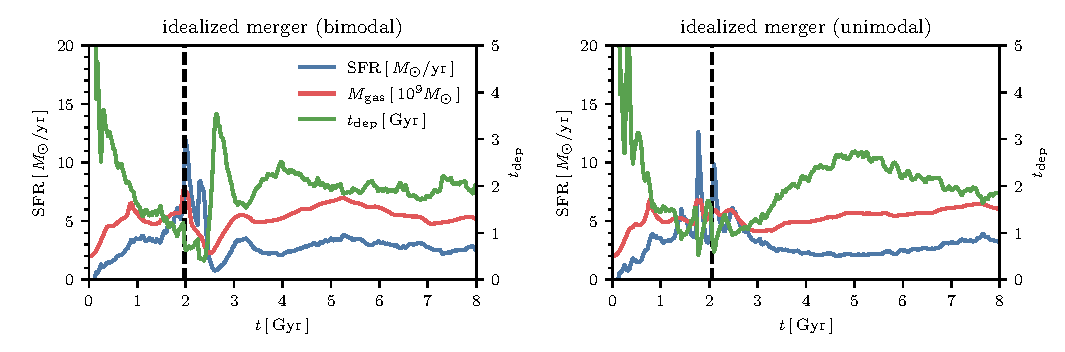
\includegraphics[width=\textwidth]{SFR_Mgas_tdep.pdf}
  \caption{\textbf{The suppression of star formation in the bimodal simulation is associated with both a reduction in gas mass as well as an increase in the depletion time.} The drop in star formation (blue line) at $\sim2.5-3\,\Gyr$ is associated with both a reduction in the total gas mass (red line) as well as an increase in the depletion time (green line). This shows that the SFR suppression is a result of both less gas mass and more inefficient star formation. \red{Should this only include the bimodal? Also, move to appendix?}}
  \label{fig:SFR_Mgas_tdep}
\end{figure*}

\begin{figure}
  \centering
  \includegraphics[width=242.26653pt]{MdotBH_rsep.pdf}
  \caption{\textbf{The bimodal merger is associated with high accretion rates onto the central SMBH.} Around the time of each pericentric passage, and slightly after, the accretion rate (blue line) becomes very high. Here, it is shown as a fraction of the Eddington accretion rate. During the merger, the accretion rate reaches as high as Eddington at some times, but is always above $10\%$. The orbital separation between the central and satellite is shown in the orange line.}
  \label{fig:MdotBH_rsep}
\end{figure}

\end{document}
